\documentclass[11pt,a4paper]{article}

\usepackage[T1]{fontenc}
\usepackage[utf8]{inputenc}
\usepackage[english]{babel}
\usepackage{lmodern}
\usepackage{amsmath,amssymb}
\usepackage{graphicx}
\usepackage{booktabs}
\usepackage{microtype}
\usepackage[margin=2.4cm]{geometry}
\usepackage[hidelinks]{hyperref}
\usepackage{natbib}
\bibliographystyle{plainnat}

\graphicspath{{figures/}}

\title{\textbf{From Quantum Decoherence to Social Polarisation}\\[2mm]
       \large A Thermodynamic Model of Public Opinion\\
       and a Proposed Metrological Index}
\author{Sylvain Geffroy}
\date{August 2026 --- \emph{working paper, open to review}}

\begin{document}
\maketitle

\begin{abstract}
\noindent
The larger a quantum system, the faster it decoheres. The larger a population, the harder
it is to reach agreement. This note formalises the structural analogy between these two
phenomena and tests its consequences numerically.

With the Helmholtz free energy $F = E - TS$ written out in full, the stationary opinion
distribution exhibits a \emph{phase transition}: above a critical social temperature, a
single peak centred on moderation; below it, two extreme peaks. Below that temperature,
removing the media field does not restore neutrality --- group conformity sustains a
\emph{hysteresis}, which explains the ineffectiveness of passive retraction. Finally, when
algorithmic gain exceeds a piece of content's natural damping rate
($\gamma\alpha > \lambda$), effective damping becomes negative and the system enters
resonance --- an informational Larsen effect.

We derive two instruments: the \textbf{Entropic Dissipation Index} (EDI), an auditable
metric of a feed's informational diversity, and the \textbf{Entropic Dissipation
Algorithm} (EDA), a recommender filter that optimises this index rather than raw
engagement.

Section~\ref{sec:limits} states the work's limitations, chief among them that the
parameters have no empirical calibration procedure. All code, tests and figures are
reproducible in containers.
\end{abstract}

\section{Introduction and hypothesis}

Sociophysics has applied the tools of statistical physics to opinion dynamics since the
1980s \citep{galam2004,castellano2009}. This note starts from a narrower and more precise
observation.

In quantum mechanics, an isolated system exists in a superposition of states. On contact
with an environment it becomes entangled with it and the interference terms vanish: this is
decoherence \citep{zeh1970,zurek2003}. The more massive the environment, the faster the
process.

The working hypothesis is:

\begin{quote}
Increasing the size of a system ($N \to \infty$) destroys the coherence of its initial
state --- in quantum physics by accelerating decoherence, in opinion dynamics by making
organic consensus unreachable.
\end{quote}

The hypothesis is \emph{structural}: it claims that one formalism describes both
situations, not that human opinion obeys physical law. Its value lies in yielding
measurable quantities. As we shall see (\S\ref{sec:limits}), it nonetheless requires an
important reformulation: the effect of $N$ is not to add disorder, but to remove
plasticity.

\section{Entropic formalism}

\subsection{Two entropies, one quantity}

The von Neumann entropy \citep{vonneumann1932}
\begin{equation}
S(\rho) = -\operatorname{Tr}(\rho \ln \rho)
\end{equation}
vanishes for a pure state. It is computed by diagonalisation: the eigenvalues of $\rho$
form a classical distribution to which the Shannon entropy \citep{shannon1948} applies,
\begin{equation}
H(X) = -\sum_i p_i \log_2 p_i .
\end{equation}
This is precisely what licenses the bridge between the two disciplines: von Neumann entropy
\emph{is} the Shannon entropy of the mixture revealed in the eigenbasis.

\subsection{A necessary clarification}

One common and incorrect formulation must be set aside at once. The evolution of a
\emph{closed} quantum system is unitary, so its von Neumann entropy is constant. What grows
under decoherence is the entropy of the \emph{reduced subsystem}, obtained by tracing over
environmental degrees of freedom.

A clarification follows that strengthens the analogy rather than weakening it: a coherent
superposition is a \emph{pure} state of zero entropy. It is therefore not the multiplicity
of possibilities that produces disorder, but the loss of coherence between them. The social
counterpart is more accurate this way: a population where everyone keeps several opinions
open is not disordered --- disorder arises from contact with an environment that fixes
positions.

\section{Thermodynamic dynamics}

\subsection{The Ising model and social temperature}

Each individual carries a binary opinion $s_i \in \{-1,+1\}$ and the population follows the
Gibbs-Boltzmann distribution \citep{ising1925}:
\begin{equation}
P(\sigma) = \frac{1}{Z}
\exp\!\left(\frac{J \sum_{\langle i,j\rangle} s_i s_j + H \sum_i s_i}{k_B T}\right),
\end{equation}
where $J$ measures local conformity, $T$ is the \emph{social temperature} (agitation,
irrationality, openness to fluctuation) and $H$ the external media field.

The model's value lies not in the analogy but in a verifiable property: the existence of a
critical temperature. In two dimensions its exact value is known \citep{onsager1944}:
\begin{equation}
\frac{T_c}{J} = \frac{2}{\ln(1+\sqrt{2})} \approx 2.269 .
\label{eq:onsager}
\end{equation}

This is the only point in this work where an exact theoretical prediction, independent of
our sociological assumptions, can validate the implementation.
Figure~\ref{fig:transition} recovers it numerically; the residual gap is a finite-size
effect on a $24\times24$ lattice.

\begin{figure}[t]
\centering
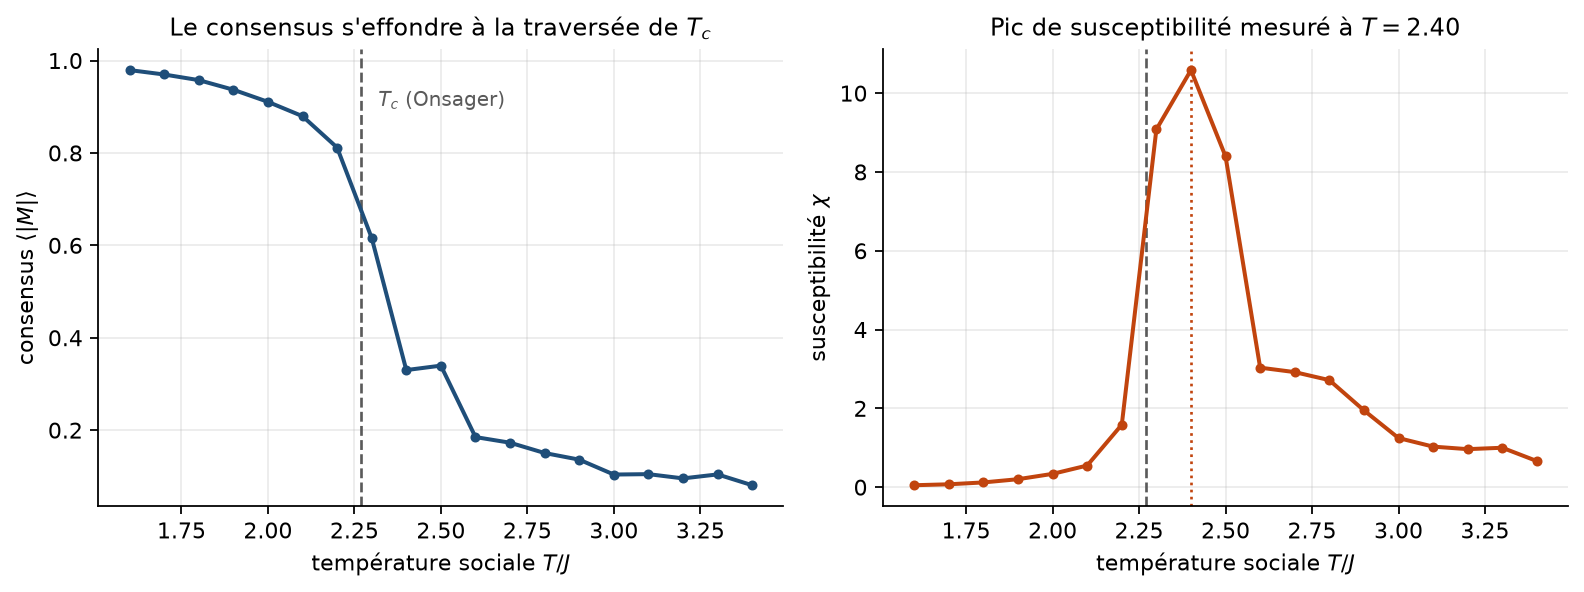
\includegraphics[width=\linewidth]{fig02_transition.png}
\caption{Consensus and susceptibility as functions of social temperature (Monte Carlo,
$24\times 24$ lattice). The susceptibility peak locates the transition. Its upward shift
relative to Onsager's value~\eqref{eq:onsager} is a finite-size effect, not an
implementation error. Figure captions are in English; notebook prose is in French.}
\label{fig:transition}
\end{figure}

\subsection{Free energy}

The system minimises its Helmholtz free energy $F = E - TS$, where $E$ represents the
tension of disagreement and $TS$ the dispersive force. As $N$ grows, configurational
entropy grows with it and the $TS$ term eventually dominates $E$.

\subsection{Social hysteresis}

This is the most directly actionable result. Below $T_c$, switching off the media field
($H \to 0$) does not return magnetisation to zero: the interaction term $-J\sum s_i s_j$
takes over and the group sustains the belief through internal cohesion.

The cycle reads in three stages, which are those of a media crisis: injection of a massive
field, official retraction, then the need for a counter-field $-H$ exceeding the group's
coercive field. Figure~\ref{fig:hysteresis} shows the cycle area decreasing with social
temperature and vanishing above $T_c$.

\begin{figure}[t]
\centering
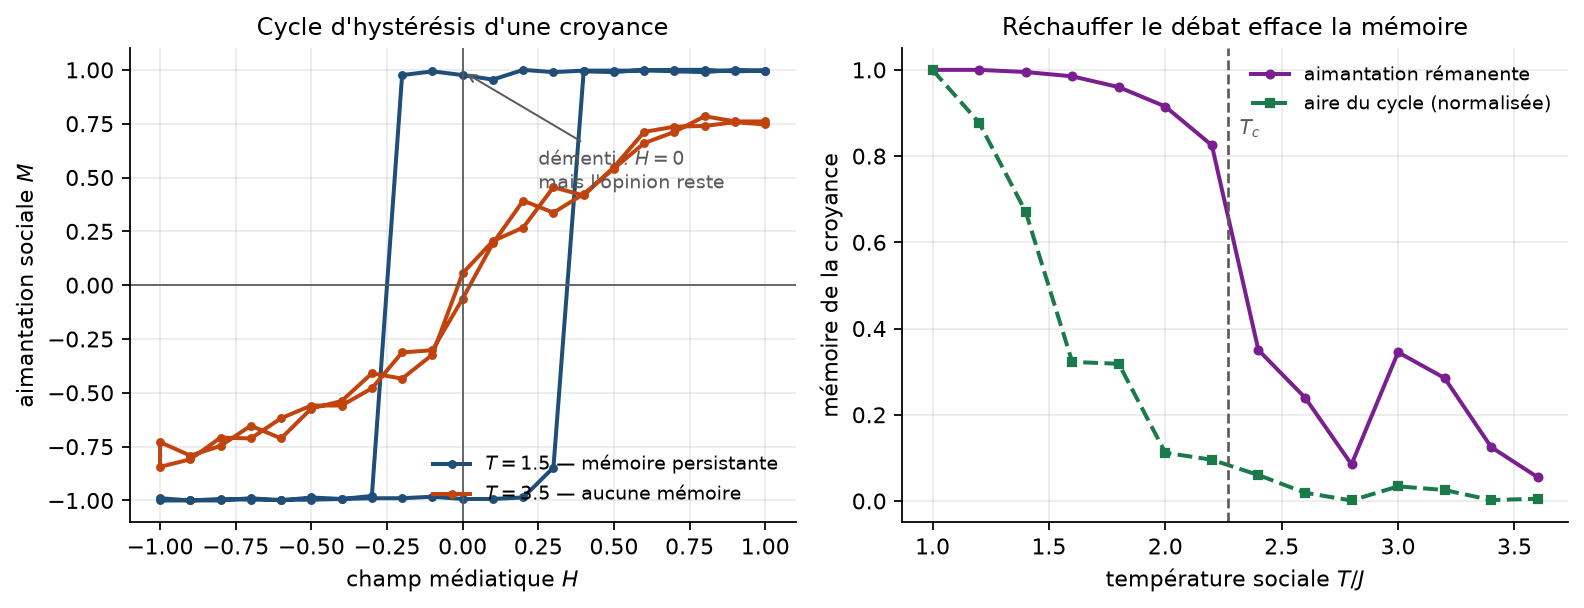
\includegraphics[width=\linewidth]{fig05_hysteresis.png}
\caption{Left: hysteresis cycles below and above $T_c$; in the former, opinion remains
magnetised while the field is zero. Right: decay of belief memory with social temperature
--- the basis for the thermal-noise recommendation.}
\label{fig:hysteresis}
\end{figure}

\emph{Practical consequence:} passive debunking does not work. Restoring informational
neutrality leaves the belief in place; only active counter-information, or a rise in social
temperature, dissipates it.

\section{Size effects: consensus time}

The voter model \citep{clifford1973,holley1975} isolates pure social contagion, without
temperature: at each interaction an individual adopts a randomly chosen neighbour's
opinion. It yields exact scaling laws for consensus time, measured in sweeps ($N$
elementary interactions).

Measurements (figure~\ref{fig:consensus}) give an exponent $\approx 1$ in mean field and
$\approx 2$ on a ring. \textbf{A densely connected network therefore converges faster than
a geographic neighbourhood.}

This invalidates a frequent argument, that the small-world structure of social networks
\citep{watts1998} prevents consensus. Connectivity does not fragment: it accelerates and
amplifies, in whatever direction the field gives it. The causes of fragmentation are the
\emph{directional bias} of algorithmic micro-fields and the \emph{homophily} that
compartments the graph \citep{pariser2011}. The regulatory consequence is clear: the useful
lever acts on the field, not on the number of links.

\begin{figure}[t]
\centering
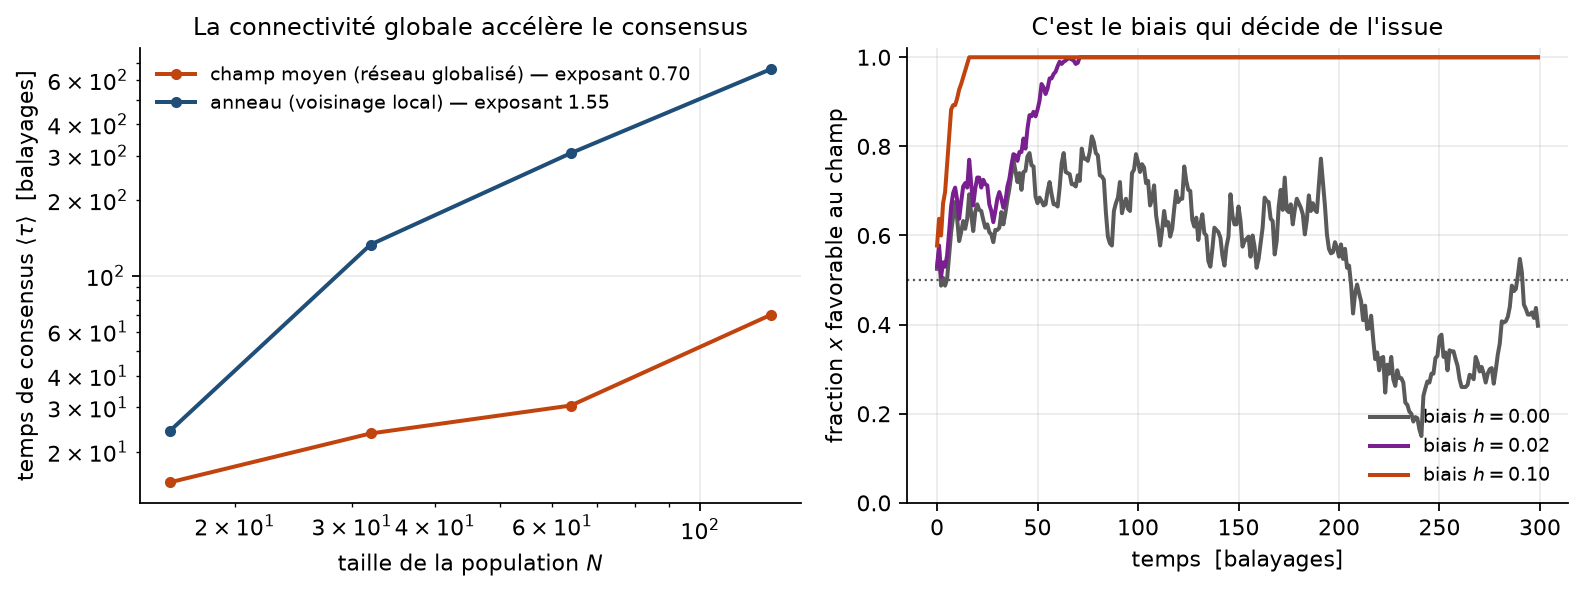
\includegraphics[width=\linewidth]{fig03_consensus.png}
\caption{Left: consensus time versus population size, log-log, for two topologies. Right:
trajectories of the field-favouring fraction for three bias intensities --- it is bias, not
connectivity, that decides the outcome.}
\label{fig:consensus}
\end{figure}

\section{The landscape of public opinion}

\subsection{The equation and its drift}

At macroscopic scale, collective opinion $x \in [-1,1]$ obeys a Fokker-Planck equation
\citep{risken1989}:
\begin{equation}
\frac{\partial P(x,t)}{\partial t}
= -\frac{\partial}{\partial x}\big[A(x)P(x,t)\big]
+ \frac{\partial^2}{\partial x^2}\big[B(x)P(x,t)\big].
\end{equation}

The quadratic potential $V(x) = -\frac{J}{2}x^2 - Hx$, which comes naturally to mind, can
produce \emph{no} phase transition: the corresponding exponential is convex, hence maximal
at the extremes at any temperature. The missing term is the entropy of mixing --- the number
of individual configurations compatible with a mean opinion $x$. Adding it recovers the
Helmholtz free energy:
\begin{equation}
f(x) = \underbrace{-\frac{J}{2}x^2 - Hx}_{E}
+ T\underbrace{\left[\frac{1+x}{2}\ln\frac{1+x}{2}
+ \frac{1-x}{2}\ln\frac{1-x}{2}\right]}_{-S},
\label{eq:free}
\end{equation}
giving the drift
\begin{equation}
A(x) = -f'(x) = Jx + H - T\operatorname{artanh}(x).
\label{eq:drift}
\end{equation}
The entropic restoring term bounds the dynamics within $(-1,1)$ and yields a mean-field
critical temperature $T_c = J$. The form $A(x) = Jx + H$ is its linearisation near $x = 0$.

\subsection{Diffusion and the effect of $N$}

The diffusion term reads
\begin{equation}
B(x) = \frac{k_B T (1-x^2)}{N},
\label{eq:diffusion}
\end{equation}
the factor $(1-x^2)$ switching off noise at unanimity.

The $1/N$ factor requires careful reading, since it appears to contradict the initial
hypothesis: the larger the population, the \emph{less} noisy its macroscopic variable.
There is no contradiction, but two distinct scales. Total configurational entropy is
extensive and grows as $N$; fluctuations of the mean $x$ decay as $1/N$. The defensible
thesis is therefore:

\begin{quote}
A large population does not become noisy, it becomes \emph{rigid}. Its size does not
agitate it; it deprives it of stochastic plasticity --- and it is that rigidity which makes
polarisation irreversible, since a system without noise can no longer leave the potential
well it has fallen into.
\end{quote}

This reformulation is stronger than the initial hypothesis: it explains irreversibility,
which the "entropy pump" metaphor did not.

\subsection{Three regimes}

The equilibrium distribution takes the large-deviation form
$P_{\mathrm{stat}}(x) \propto \exp(-N f(x)/T)$, where the factor $N$ makes the penalty more
severe the larger the population. Three regimes follow, obtained by varying two parameters
(figure~\ref{fig:landscape}): a fluid society ($T > T_c$), a polarised one ($T < T_c$,
$H = 0$) and a manipulated one ($T < T_c$, $H > 0$). In the last case the peak on the
field's side overwhelms the other: the "false consensus" is not an added assumption, it is
the tilted well.

The density of moderates decays exponentially with $N$. In a large population below $T_c$,
moderation is not a minority position: it is statistically inaccessible.

\begin{figure}[t]
\centering
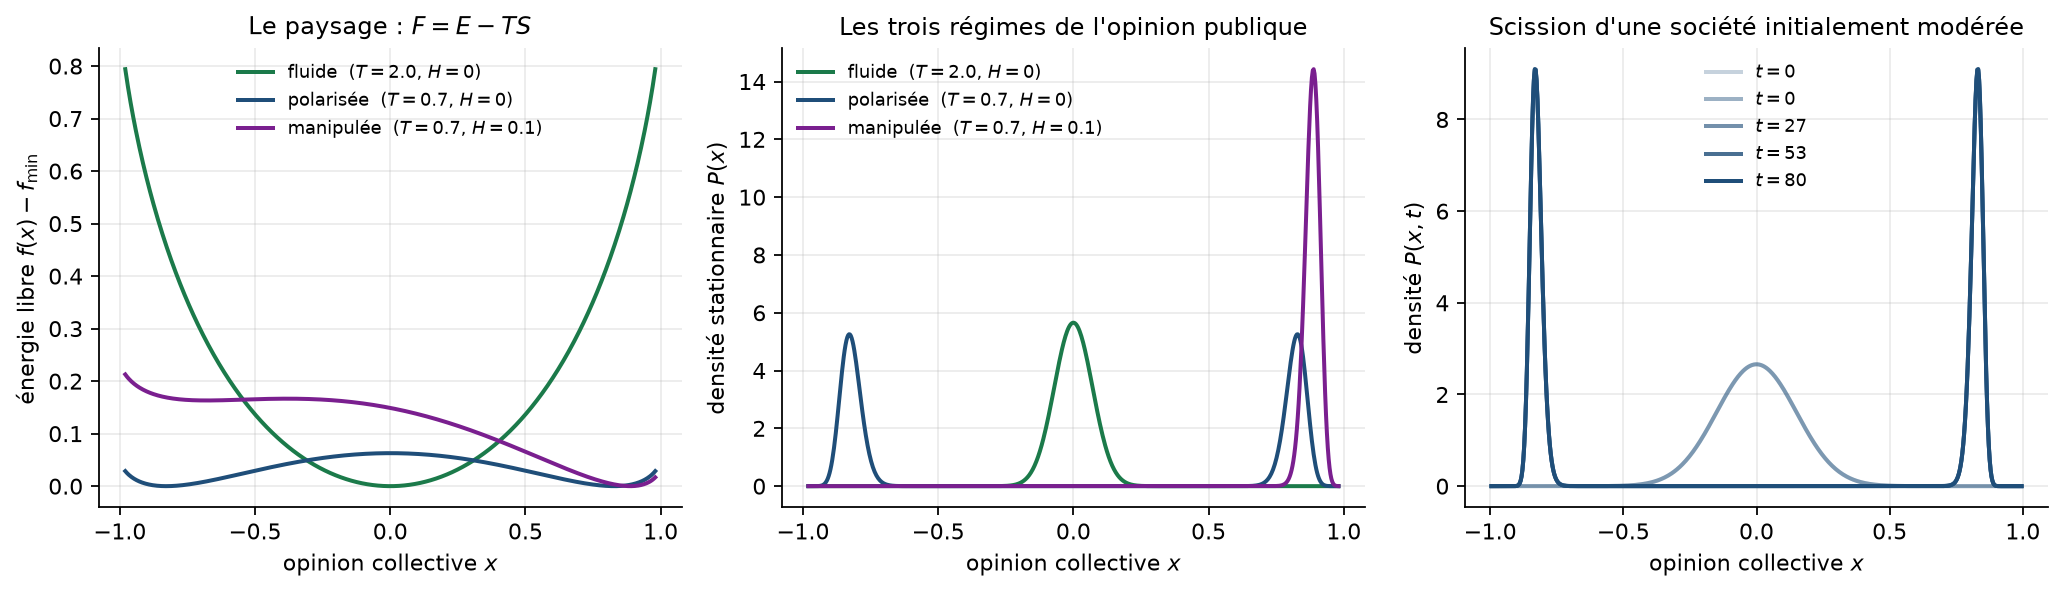
\includegraphics[width=\linewidth]{fig04_paysage.png}
\caption{Free-energy landscape~\eqref{eq:free}, the associated stationary distributions, and
the temporal splitting of an initially moderate society. The solver uses finite volumes with
zero flux at the boundaries: probability mass is conserved to $10^{-15}$, which distinguishes
a genuine collapse of moderation from numerical leakage.}
\label{fig:landscape}
\end{figure}

\subsection{Barrier crossing}

Moving from one bloc to the other without passing through moderation is thermally activated
barrier crossing, with rate $\propto e^{-\Delta V / k_B T}$ \citep{kramers1940}, and not
tunnelling --- which has no classical counterpart. The distinction is not cosmetic:
Kramers' law supplies a temperature dependence, hence a testable prediction.

\section{Algorithmic resonance kinetics}

A piece of false information and a recommender algorithm form a positive feedback loop
analogous to the Larsen effect. Visibility $V(t)$ obeys
\begin{equation}
\ddot V + \big(\lambda - \gamma\alpha\,\sigma(V)\big)\dot V + \omega_0^2 V = \xi(t),
\label{eq:resonance}
\end{equation}
where $\lambda$ is natural damping (forgetting), $\gamma$ the algorithmic gain, $\alpha$ the
content's emotional charge, and $\sigma(V) = 1/(1+(V/V_{\mathrm{sat}})^2)$ a saturation
factor expressing the finiteness of available attention.

The instability criterion is
\begin{equation}
\boxed{\;\gamma\alpha > \lambda\;}
\label{eq:criterion}
\end{equation}
Beyond it, effective damping becomes negative: the system accumulates energy instead of
dissipating it. Figure~\ref{fig:resonance} confirms that the measured threshold coincides
with $\gamma^\star = \lambda/\alpha$.

Without saturation the unstable solution diverges as $e^{(\gamma\alpha-\lambda)t}$, which is
exact but unusable: infinite visibility does not exist and no threshold is calibratable on a
divergent model. With saturation the system settles into a limit cycle --- a self-sustaining
media oscillation of finite amplitude, matching the observed behaviour of established
disinformation.

\begin{figure}[t]
\centering
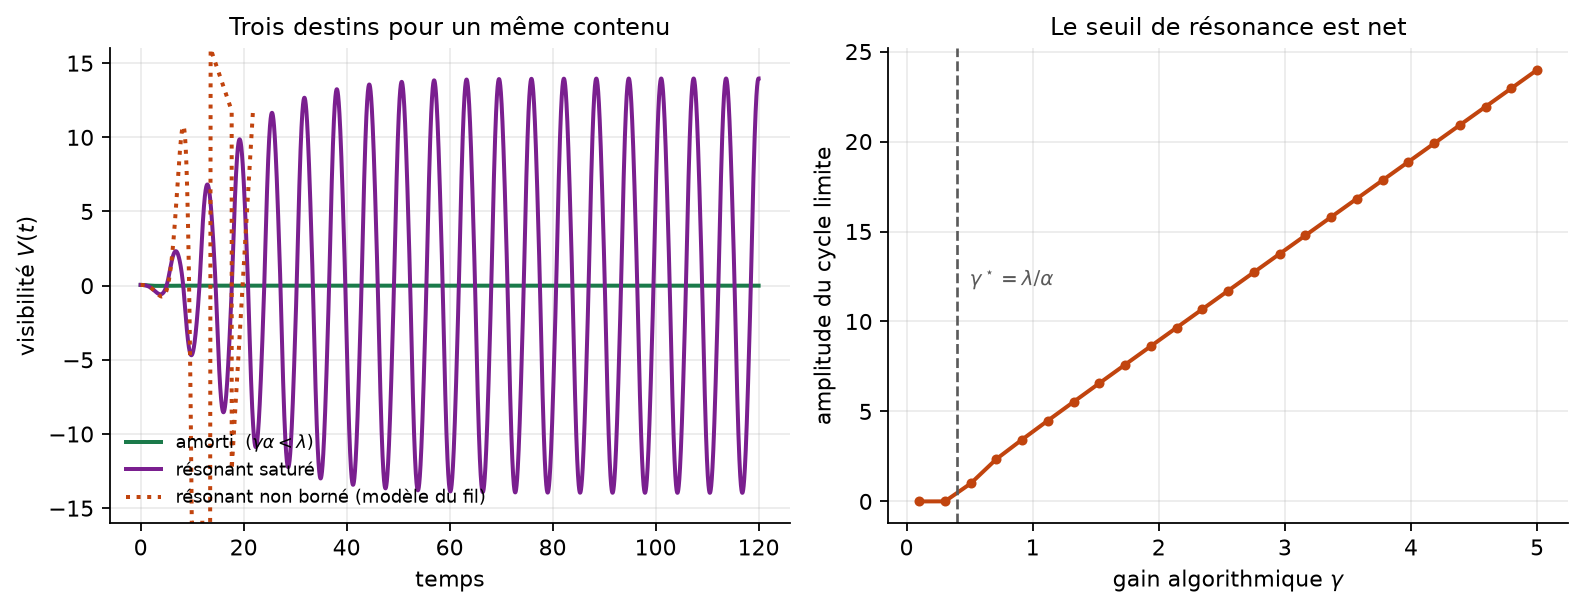
\includegraphics[width=\linewidth]{fig06_resonance.png}
\caption{Left: three fates for the same content --- damped, bounded resonant, unbounded
resonant. Right: limit-cycle amplitude versus algorithmic gain; the measured threshold
coincides with $\gamma^\star = \lambda/\alpha$.}
\label{fig:resonance}
\end{figure}

One point deserves emphasis for regulation. At \emph{uniform} gain, a more emotional item
crosses the threshold where a factual one does not. A platform therefore need not favour
disinformation in order to amplify it selectively: the bias is mechanical. This is what
makes measuring $\gamma$ more relevant, and more enforceable, than auditing editorial
intent.

\section{Two instruments}

\subsection{The Entropic Dissipation Index}

The index is the Shannon entropy of the viewpoints served to a user, normalised by its
theoretical maximum:
\begin{equation}
\mathrm{EDI} = \frac{H(X)}{\log_2 k} \in [0,1].
\label{eq:edi}
\end{equation}
Normalisation is the essential point: it makes the index dimensionless and comparable across
platforms, which a threshold in bits does not. The denominator $k$ --- the number of
viewpoints the platform is \emph{able} to serve --- must be imposed by the regulator, failing
which a perfectly closed feed would obtain a flattering index.

A collapsed index is the signature of a zero local social temperature, that is, a frozen
state in the Ising sense --- the regime in which hysteresis makes false beliefs persistent.

\subsection{The Entropic Dissipation Algorithm}

A conventional recommender maximises immediate engagement; by \eqref{eq:criterion}, that
cost function is the one producing negative damping. The algorithm replaces it with
\begin{equation}
S(i,c) = \mathrm{Relevance}(i,c) + \mu \cdot \Delta H(i,c),
\qquad \mu \geq 0,
\label{eq:eda}
\end{equation}
where $\Delta H = H_{\mathrm{future}} - H_{\mathrm{current}}$ measures the item's impact on
the feed's index. The positive sign is essential: it rewards diversification. The relevance
term is retained --- an algorithm serving diversity without relevance would be abandoned by
its users, dissipating no entropy at all.

The coefficient $\mu$ is not constant. It stays at a resting value while the index is
satisfactory, and rises progressively once the index falls below the critical threshold: this
transposes simulated annealing, a temperature spike to break a frozen state followed by
cooling. At $\mu = 0$ the algorithm is indistinguishable from an engagement filter, which
makes it a parameterised addition rather than a redesign.

\section{Limitations}
\label{sec:limits}

These are stated here rather than left to reviewers.

\paragraph{No empirical calibration.} This is the principal weakness. The parameters $J$,
$T$, $\gamma$, $\alpha$ have no estimation procedure on real data. The formalism is
coherent; its empirical grounding remains to be built. The most accessible route would be
estimating $\gamma\alpha/\lambda$ by fitting \eqref{eq:resonance} to public visibility time
series.

\paragraph{An analogy is not an explanation.} Nothing here demonstrates that opinion
\emph{obeys} statistical mechanics. The work establishes that a formalism borrowed from
physics \emph{reproduces} certain observed behaviours. Kramers' prediction on the temperature
dependence of switching rates would offer a falsifiable test; it has not been carried out.

\paragraph{Individuals are not spins.} Intentionality, irony and strategic contrarianism have
no counterpart in a spin model. Opinions are multidimensional --- the agent model uses two
continuous axes, which mitigates the problem without solving it \citep{deffuant2000}.
Finally, the environment is not passive: an algorithm optimises a cost function, making it a
strategic actor rather than a thermal bath. This is the analogy's weakest point, and it is
also what makes the algorithm conceivable --- a cost function can be changed.

\paragraph{Limitations specific to the index as an instrument.} Discretisation into viewpoints
is a political choice: whoever defines the modalities defines the index. The index is
gameable, since a platform can serve formally divergent but substantively empty content.
Measuring it on individual feeds raises a privacy question this work does not answer. And
imposing an index floor is a constraint on what citizens see: defensible, but an intervention
in public debate, and presenting it as a neutral technical measure would be dishonest.

\paragraph{Scope of the simulations.} The regimes explored were chosen for legibility. No
systematic sensitivity study was carried out, system sizes are modest, and no result is
compared against real data. The conclusions are qualitative: they concern the existence of
regimes and the direction of dependencies, never transposable numerical values.

\section{Reproducibility}

The complete work is openly available, runnable in containers, with $203$ automated tests.
The structuring verifications cover Onsager's critical temperature~\eqref{eq:onsager}, exact
conservation of probability mass, the exponents of consensus-time scaling laws, the strict
positivity of the hysteresis cycle area below $T_c$, and the equivalence of the algorithm
with an engagement filter at $\mu = 0$. Every figure in this note is regenerated by a
notebook.

\begin{center}
\url{https://github.com/s-geffroy/Index-Dissipation-Entropique}\\
\url{https://s-geffroy.github.io/Index-Dissipation-Entropique/en/}
\end{center}

This work is open to critical review. Feedback on empirical calibration, on the index's
viability as a regulatory instrument, or on remaining analogies that do not hold, is the most
valuable.

\bibliography{refs}

\end{document}
